\documentclass[8pt,xcolor={dvipsnames}]{beamer}

% handout
% \documentclass[handout, 10pt]{beamer}

\usepackage{clases}

\title{Investigación Operativa}
\subtitle{Redes de flujo - Problemas de flujo m\'aximo}
\date{}
\author{Facundo Gutiérrez - Nazareno Faillace}
\institute{Departamento de Matemática, FCEN, UBA}
% \titlegraphic{\hfill\includegraphics[height=1.5cm]{logo.pdf}}

\newcommand \anchoPagina{1.0} % El proyector no anda bien, hay que ajustar el ancho
\begin{document}

\maketitle

\section{Red de flujo}

\begin{frame}{Definici\'on de flujo}
	Una \textit{red de flujo} es un grafo dirigido $\mathcal{G} = (\mathbb{V},\mathbb{E},c)$ donde $c : \mathbb{E} \to \mathbb{R}_{\geq 0}$ es una funci\'on que a cada arista le asigna un n\'umero que llamamos \textit{capacidad}.
	
	Vamos a distinguir dos nodos del grafo, $s,t \in \mathbb{V}$ que llamaremos \textit{fuente} y \textit{sumidero}. Usualmente, no llegan aristas a $s$ y no salen aristas de $t$.
	
	\pause
	Dada una red de flujo, decimos que una funci\'on $f : \mathbb{E} \to \mathbb{R}$ es un \textit{flujo} si satisface:
	\begin{enumerate}
		\item $f(e) \leq c(e) \quad \forall e \in \mathbb{E}$
		\item $\sum\limits_{e=(v,u) \in \mathbb{E}} f(e) = \sum\limits_{e=(u,v) \in \mathbb{E}} f(e) \quad \forall v \in \mathbb{V}\setminus \{s,t\}$
	\end{enumerate} 
	
	Dado, un flujo definimos a su \textit{valor} como $$|f| = \sum\limits_{e=(s,u) \in \mathbb{E}} f(e) \underset{\text{esto es $0$ si no llegan aristas a }s}{-\underbrace{\sum\limits_{e = (u,s) \in \mathbb{E}} f(e)}}$$
	
\end{frame}

\begin{frame}{Problema de m\'aximo flujo}
	Durante esta clase discutiremos el problema de obtener un \textit{flujo de valor m\'aximo} para una red de flujo dada.
	
	Veamos un ejemplo de las definiciones anteriores. Para un flujo $f$, se utiliza la notaci\'on $f(e) / c(e)$ sobre cada arco para indicar los valores correspondientes a $f$ y $c$.
	\pause
	\begin{center} 
		\begin{tikzpicture}[
		mycircle/.style={
			circle,
			draw=black,
			fill=gray,
			fill opacity = 0.3,
			text opacity=1,
			inner sep=0pt,
			minimum size=20pt,
			font=\small},
		myarrow/.style={-Stealth},
		node distance=0.6cm and 1.2cm
		]
		\node[mycircle] (c1) {$s$};
		\node[mycircle,below right=of c1] (c2) {$v_2$};
		\node[mycircle,right=of c2] (c3) {$v_4$};
		\node[mycircle,above right=of c1] (c4) {$v_1$};
		\node[mycircle,right=of c4] (c5) {$v_3$};
		\node[mycircle,below right=of c5] (c6) {$t$};
		
		\foreach \i/\j/\txt/\p in {% start node/end node/text/position
			c1/c2/\text{8/13}/below,
			c1/c4/\text{11/16}/above,
			c2/c3/\text{11/14}/below,
			c3/c6/\text{4/4}/below,
			c4/c5/\text{12/12}/above,
			c5/c6/\text{15/20}/above,
			c5/c2/\text{4/9}/below,
			c3/c5/\text{7/7}/below,
			c2.70/c4.290/\text{1/4}/below}
		\draw [myarrow] (\i) -- node[sloped,font=\small,\p] {\txt} (\j);
		
		
		% draw this outside loop to get proper orientation of 10
		\draw [myarrow] (c4.250) -- node[sloped,font=\small,above,rotate=180] {\text{0/10}} (c2.110);
		\end{tikzpicture}
	\end{center} 
	\pause
	
	¿Podemos mejorarlo?
\end{frame}

\begin{frame}{Problema de m\'aximo flujo - Red Residual}
	Dada una funci\'on de flujo $f$, para saber si podemos encontrar un nuevo flujo de $s$ a $t$ con mayor valor, se construye una nueva red que se denomina \textit{red residual}. En esta nueva red cada arco expresa c\'omo podemos cambiar el flujo actual. Tiene los mismos v\'ertices, pero por cada arista $e = (u,v) \in \mathbb{E}$ se tienen hasta dos aristas.
	\begin{itemize}
		\item $\hat{e}_1 = (u,v)$ con capacidad de cambio $c(e) - f(e)$, si $c(e) - f(e) > 0$
		\item $\hat{e}_2 = (v,u)$ con capacidad de cambio $f(e)$, si $f(e) > 0$
	\end{itemize}
	\pause
	A un camino simple de $s$ a $t$ en esta red, se lo denomina un \textit{camino de aumento}. La raz\'on de este nombre es que dado un camino de aumento, se puede construir un nuevo flujo a partir de $f$, cuyo valor aumentar\'a tanto como la arista de \textit{menor} capacidad de cambio en el camino de aumento.
	
\end{frame}

\begin{frame}{Problema de m\'aximo flujo - Red Residual}
	\begin{center} 
		\begin{tikzpicture}[
		mycircle/.style={
			circle,
			draw=black,
			fill=gray,
			fill opacity = 0.3,
			text opacity=1,
			inner sep=0pt,
			minimum size=20pt,
			font=\small},
		myarrow/.style={-Stealth},
		node distance=0.6cm and 1.2cm
		]
		\node[mycircle] (c1) {$s$};
		\node[mycircle,below right=of c1] (c2) {$v_2$};
		\node[mycircle,right=of c2] (c3) {$v_4$};
		\node[mycircle,above right=of c1] (c4) {$v_1$};
		\node[mycircle,right=of c4] (c5) {$v_3$};
		\node[mycircle,below right=of c5] (c6) {$t$};
		
		\foreach \i/\j/\txt/\p in {% start node/end node/text/position
			c1/c2/\text{8/13}/below,
			c1/c4/\text{11/16}/above,
			c2/c3/\text{11/14}/below,
			c3/c6/\text{4/4}/below,
			c4/c5/\text{12/12}/above,
			c5/c6/\text{15/20}/above,
			c5/c2/\text{4/9}/below,
			c3/c5/\text{7/7}/below,
			c2.70/c4.290/\text{1/4}/below}
		\draw [myarrow] (\i) -- node[sloped,font=\small,\p] {\txt} (\j);
		
		
		% draw this outside loop to get proper orientation of 10
		\draw [myarrow] (c4.250) -- node[sloped,font=\small,above,rotate=180] {\text{0/10}} (c2.110);
		\end{tikzpicture}
		\pause
		\includegraphics<1-3>[scale = 0.25]{imagenes/red_residual_2.png}
		\includegraphics<4>[scale = 0.25]{imagenes/red_residual_3.png}
		\includegraphics<5->[scale = 0.25]{imagenes/red_residual_4.png}
	\end{center}
	\pause
	{\small
	¿Hay alg\'un camino de aumento? \pause ¿En cu\'anto se puede aumentar este nuevo flujo? \pause ¿C\'omo se actualiza la nueva red residual?}
\end{frame}

\begin{frame}{Problema de m\'aximo flujo - Red Residual}
	\begin{center} 
		\begin{tikzpicture}[
		mycircle/.style={
			circle,
			draw=black,
			fill=gray,
			fill opacity = 0.3,
			text opacity=1,
			inner sep=0pt,
			minimum size=20pt,
			font=\small},
		myarrow/.style={-Stealth},
		node distance=0.6cm and 1.2cm
		]
		\node[mycircle] (c1) {$s$};
		\node[mycircle,below right=of c1] (c2) {$v_2$};
		\node[mycircle,right=of c2] (c3) {$v_4$};
		\node[mycircle,above right=of c1] (c4) {$v_1$};
		\node[mycircle,right=of c4] (c5) {$v_3$};
		\node[mycircle,below right=of c5] (c6) {$t$};
		
		\foreach \i/\j/\txt/\p in {% start node/end node/text/position
			c1/c2/\text{12/13}/below,
			c1/c4/\text{11/16}/above,
			c2/c3/\text{11/14}/below,
			c3/c6/\text{4/4}/below,
			c4/c5/\text{12/12}/above,
			c5/c6/\text{19/20}/above,
			c5/c2/\text{0/9}/below,
			c3/c5/\text{7/7}/below,
			c2.70/c4.290/\text{1/4}/below}
		\draw [myarrow] (\i) -- node[sloped,font=\small,\p] {\txt} (\j);
		
		
		% draw this outside loop to get proper orientation of 10
		\draw [myarrow] (c4.250) -- node[sloped,font=\small,above,rotate=180] {\text{0/10}} (c2.110);
		\end{tikzpicture}
		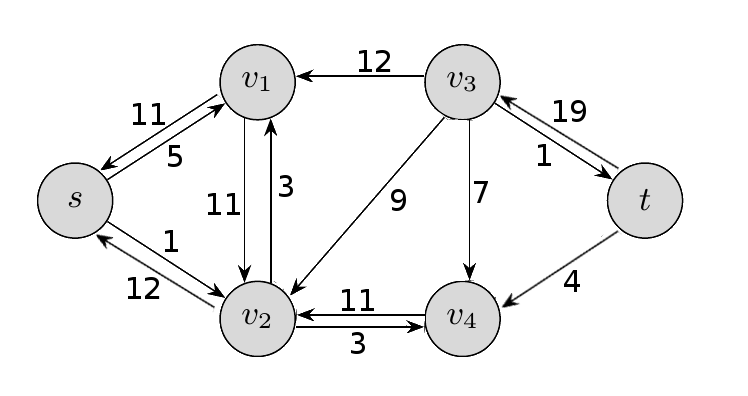
\includegraphics[scale = 0.25]{imagenes/red_residual_5.png}
	\end{center}
	{\small
	¿Hay alg\'un camino de aumento? ¿En cu\'anto se puede aumentar este nuevo flujo? ¿C\'omo se actualiza la nueva red residual?}
\end{frame}

\begin{frame}{Algunas definiciones m\'as}
	\begin{center}
		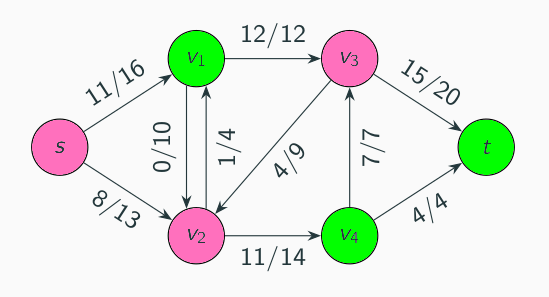
\includegraphics[scale = 0.35]{imagenes/corte.png}
	\end{center}
	Dada una red de flujo, un \textit{corte} en la red es una partici\'on de $\mathbb{V}$ en dos conjuntos, $\mathbb{S}$ y $\mathbb{T}$, de forma que $s\in \mathbb{S}$ y $t \in \mathbb{T}$. Notar que por ser una partici\'on, $\mathbb{V} = \mathbb{S} \overset{d}{\cup} \mathbb{T}$.
	\pause
	Si adem\'as de la red, tenemos un flujo factible $f$, para un corte dado podemos definir:
	\begin{itemize}
		\item El \textit{flujo neto} del corte: $f(\mathbb{S},\mathbb{T})= \sum\limits_{\substack{e = (u,v) \in \mathbb{E} \\ u \in \mathbb{S}, v \in \mathbb{T}}} f(e) - \sum\limits_{\substack{e = (u,v) \in \mathbb{E} \\ u \in \mathbb{T}, v \in \mathbb{S}}} f(e)$
		
		\item La \textit{capacidad} del corte: $c(\mathbb{S},\mathbb{T})= \sum\limits_{\substack{e = (u,v) \in \mathbb{E} \\ u \in \mathbb{S}, v \in \mathbb{T}}} c(e) $
	\end{itemize}
	\textbf{Obs:} la capacidad de un corte acota superiormente a su flujo neto: $f(\mathbb{S},\mathbb{T})= \sum\limits_{\substack{e = (u,v) \in \mathbb{E} \\ u \in \mathbb{S}, v \in \mathbb{T}}} f(e) - \sum\limits_{\substack{e = (u,v) \in \mathbb{E} \\ u \in \mathbb{T}, v \in \mathbb{S}}} f(e) \leq \sum\limits_{\substack{e = (u,v) \in \mathbb{E} \\ u \in \mathbb{S}, v \in \mathbb{T}}} f(e) \leq \sum\limits_{\substack{e = (u,v) \in \mathbb{E} \\ u \in \mathbb{S}, v \in \mathbb{T}}} c(e) = c(\mathbb{S},\mathbb{T})$

	
\end{frame}

\begin{frame}{Algoritmo de Ford Fulkerson}
	Con estas ideas en mente se tiene el siguiente algoritmo para calcular un flujo m\'aximo.
	\begin{enumerate}
		\item Comenzar con un flujo vac\'io
		\item Construir la red residual
		\item Mientras existan caminos de aumento en la red residual:
		\begin{enumerate}
			\item Incrementar el flujo por alg\'un camino de aumento
			\item Reactualizar la red residual para este nuevo flujo 
		\end{enumerate}
	\end{enumerate} 
	
	Notemos que como $c(e) \geq 0 \quad \forall e \in \mathbb{E}$, entonces el flujo vac\'io siempre es factible (el flujo vac\'io es la funci\'on $f(e) = 0 \quad \forall e \in \mathbb{E}$)
		
\end{frame}

\begin{frame}{Flujo M\'aximo - Corte Mínimio}
    \begin{tcolorbox}[title=Teorema]
        Son equivalentes:
	\begin{enumerate}
		\item $f$ es un flujo m\'aximo
		\item No hay caminos de aumento en la red residual
		\item $|f| = c(\mathbb{S},\mathbb{T})$ para alg\'un corte
	\end{enumerate}  
    \end{tcolorbox}
% 	\pause
% 	\underline{Demostraci\'on} (Idea):
% 	\begin{itemize}
% 		\item [$1\Rightarrow 2$)] Si hubiese camino de aumento, el flujo no ser\'ia m\'aximo
% 		\pause
% 		\item [$2\Rightarrow 3$)] Por hip\'otesis, en la red residual $s$ y $t$ est\'an desconectados. Tomamos $\mathbb{S}$ como los alcanzables desde $s$ en la red residual y $\mathbb{T} = \mathbb{V} \setminus \mathbb{S}$, lo cual nos define un corte. M\'as a\'un, este corte cumple $|f| = f(\mathbb{S},\mathbb{T}) = c(\mathbb{S},\mathbb{T})$
% 		\pause
% 		\item [$3\Rightarrow 1$)] Cualquier corte acota superiormente a todo flujo. Por lo tanto, el flujo en cuesti\'on debe ser m\'aximo (m\'as a\'un, como todo flujo acota inferiormente a un corte, dicho corte es m\'inimo).
% 	\end{itemize}
% 	 \pause
	 \textbf{Corolario}: El algoritmo de Ford-Fulkerson es correcto.
\end{frame}

\section{Problemas de flujo m\'aximo}

\begin{frame}{M\'ultiples fuentes o sumideros}
	Supongamos que ahora debemos enviar desde $s_1,s_2, \dots s_a$ y enviar a $t_1,t_2,\dots,t_b$. ¿C\'omo podemos reducirlo al problema que ten\'iamos antes?
	
	\visible<2>{Agregamos un v\'ertice $s$ y aristas a todas las fuentes $s_i$ de la forma  $s \to s_i$ con capacidad infinita. 
	
	Tambi\'en agregamos un v\'ertice $t$ y aristas a todas las fuentes $t_j$ de la forma  $t_j \to t$ con capacidad infinita.}
	
	\only<1>{\begin{figure}
	    \centering
	    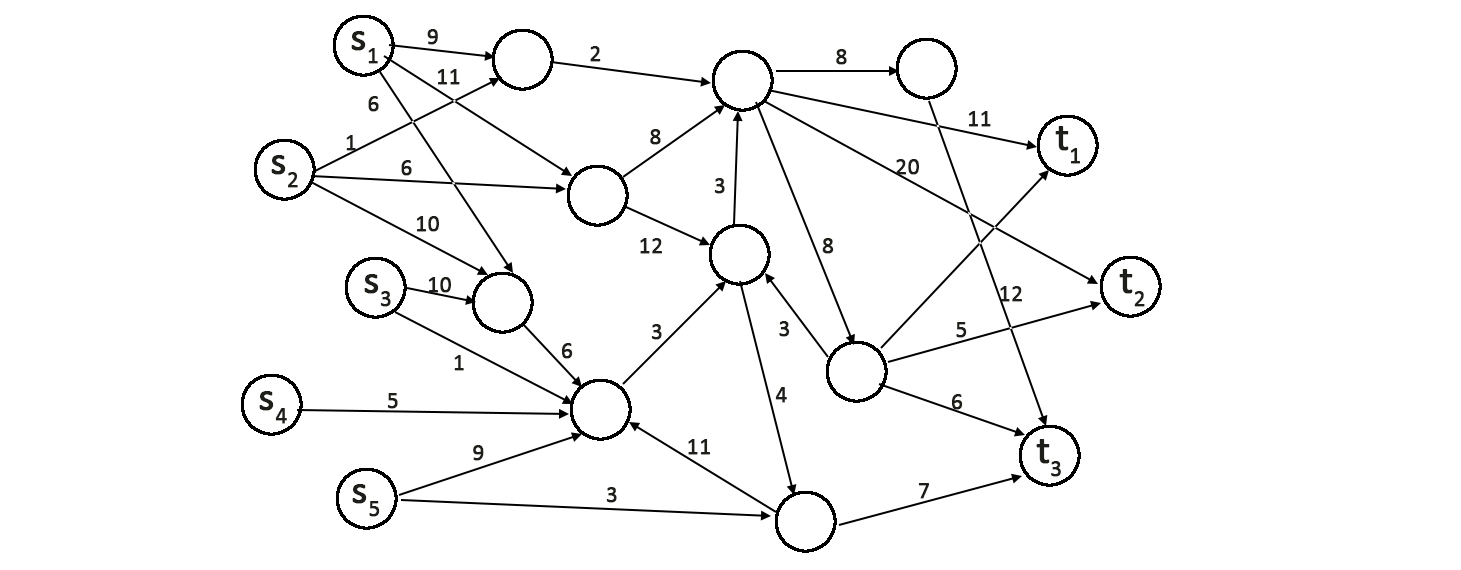
\includegraphics[width=\textwidth]{imagenes/multi1.jpg}
	\end{figure}}
	\only<2>{\begin{figure}
	    \centering
	    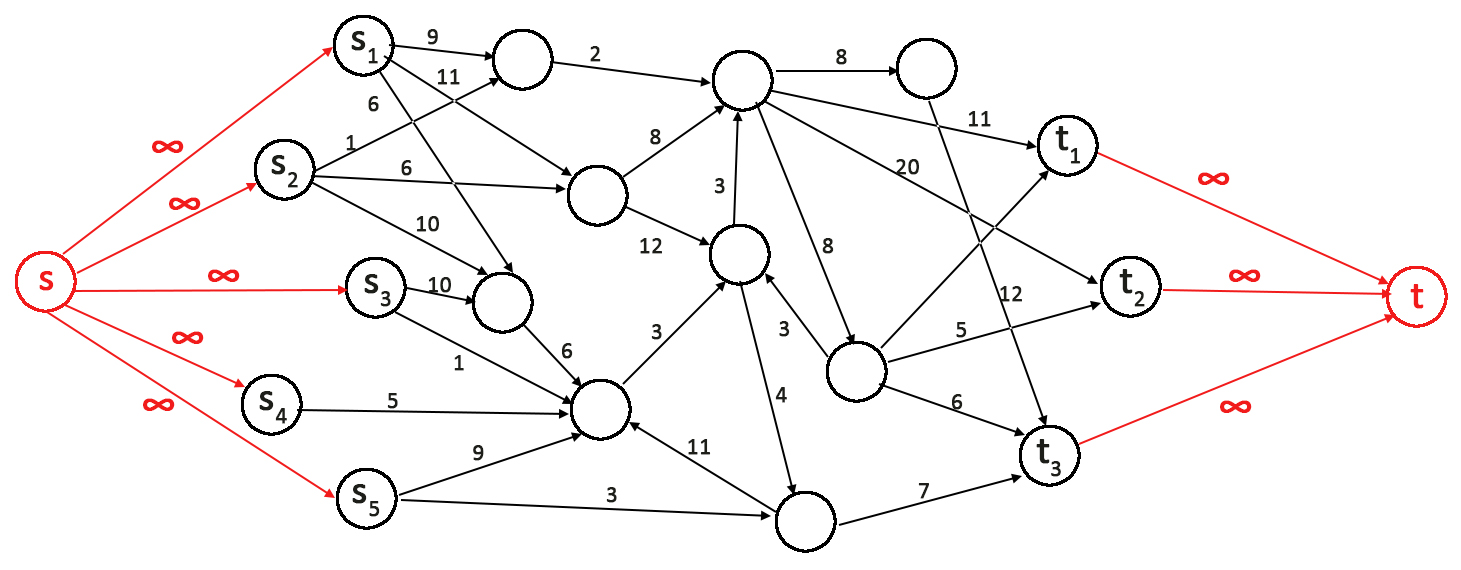
\includegraphics[width=\textwidth]{imagenes/multi2.jpg}
	\end{figure}}
\end{frame}

\begin{frame}{Capacidades en los v\'ertices}
	Si ahora nuestro problema dice que por un cierto v\'ertice no pueden pasar m\'as de $w$ unidades de flujo, ¿c\'omo lo reducimos al problema que ya sabemos resolver?
	
	\visible<2>{Lo que hacemos es \textit{separar a nuestro nodo en dos}. Si el nodo en cuesti\'on es $v$, lo separamos en $v_{in}$ y $v_{out}$. 
	
	Toda arista que antes entraba a $v$ ahora va a entrar a $v_{in}$. An\'alogamente, toda arista que antes sal\'ia de $v$, ahora va a salir de $v_{out}$.
	
	Finalmente, agregamos una arista con capacidad $w$ de la forma $v_{in} \overset{w}{\to} v_{out}$ para modelar correctamente el problema.}
	
	\only<1>{\begin{figure}
	    \centering
	    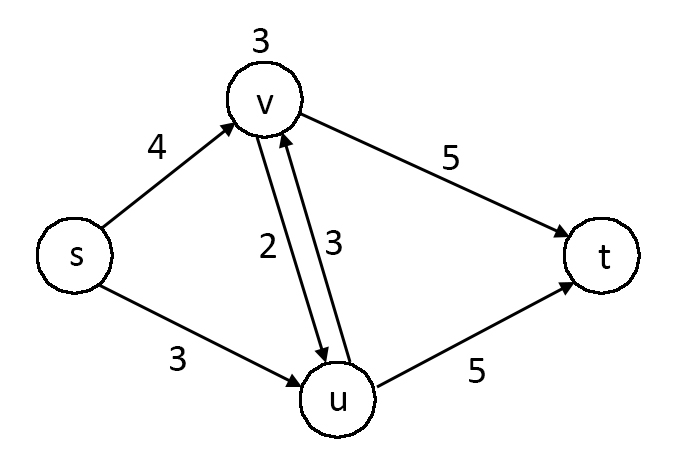
\includegraphics[scale=0.25]{imagenes/vexp1.jpg}
	\end{figure}}
	\only<2>{\begin{figure}
	    \centering
	    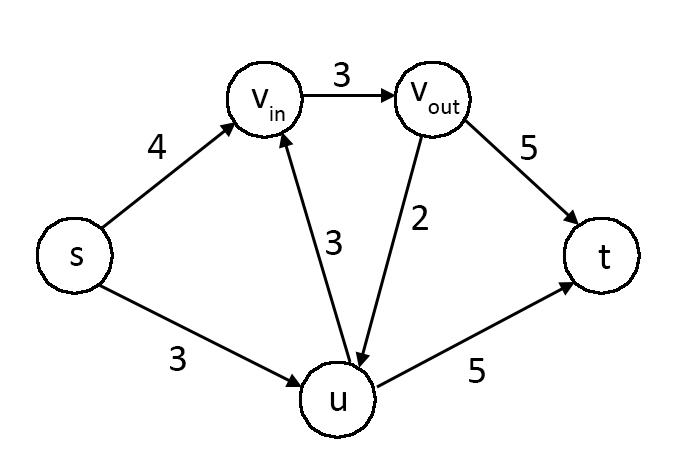
\includegraphics[scale=0.25]{imagenes/vexp2.jpg}
	\end{figure}}
\end{frame}

\begin{frame}{M\'axima cantidad de caminos disjuntos en aristas}
	Dado un grafo dirigido buscamos el m\'aximo n\'umero de caminos que comienzan en $s$ y finalizan en $t$ y adem\'as son disjuntos en aristas.
	
	\pause
	Si asignamos a cada arista una unidad capacidad (es decir $c(e) = 1 \quad \forall e \in \mathbb{E}$), luego, el m\'aximo flujo en esta red nos da la m\'axima cantidad de caminos disjuntos en aristas que pueden ubicarse en el grafo.
	\pause
	
	¿C\'omo resolver\'iamos el problema si ahora necesitamos que los caminos sean disjuntos en v\'ertices (salvo por $s$ y $t$)?
\end{frame}


\begin{frame}{Matching (en grafos bipartitos)}
	
	Dado un grafo no dirigido, un matching es un subconjunto de aristas, que cumple que para todo nodo del grafo no existen dos aristas del matching incidiendo en dicho nodo.
	
	El problema en cuesti\'on es encontrar un matching m\'aximo. Sin ninguna restricci\'on adicional, existen algoritmos polinomiales que resuelven el problema, pero en la clase de hoy nos centraremos en resolver el problema cuando el grafo en cuesti\'on es bipartito.
	
	\pause
	Si existe una bipartici\'on del grafo en $\mathbb{V}_1$ y $\mathbb{V}_2$ podemos reducir el problema de matching m\'aximo al problema anterior. 
	
	Direccionamos todas las aristas del grafo de un nodo de $\mathbb{V}_1$ a un nodo de $\mathbb{V}_2$. Agregamos al grafo un nodo $s$, y conectamos $s \overset{1}{\to} v \quad \forall v \in \mathbb{V}_1$. Si ahora agregamos $t$ un sumidero y conectamos $v \overset{1}{\to} t \quad \forall v \in \mathbb{V}_2$, entonces podemos identificar a cada matching con una partici\'on en caminos disjuntos en aristas de este grafo. 
	
\end{frame}

\begin{frame}{Matching (en grafos bipartitos)}
	\begin{center}
		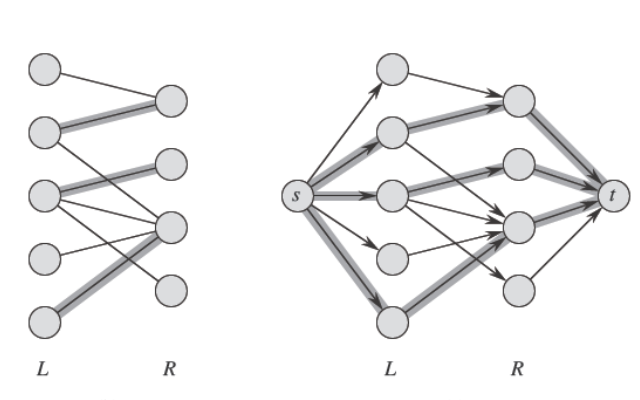
\includegraphics[scale = 0.5]{imagenes/matching_bipartito.png} 
	\end{center}
\end{frame}

\begin{frame}{Teoremas de Hall, K\H{o}nig}
	
% 	Para $\mathcal{X} \subseteq \mathbb{V}$, definimos $f(\mathcal{X}) := \underset{v \in \mathcal{X}}{\cup} \mathcal{N}(v)$.
% 	\pause
	
	\begin{tcolorbox}[title=Teorema de Hall]
	    Dado un grafo bipartito con $|\mathbb{V}_2| < |\mathbb{V}_1|$. Existe un matching cuyos extremos contienen a $\mathbb{V}_2$ en su totalidad si y solo si para todo subconjunto $\mathcal{X} \subseteq \mathbb{V}_2$ se satisface que $|\mathcal{X}| \leq |\underset{v \in \mathcal{X}}{\cup} \mathcal{N}(v)|$
	\end{tcolorbox}

	\pause
	
	Definimos a un \textit{cubrimiento de las aristas por nodos} a un subconjunto de v\'ertices $\mathcal{V} \subseteq \mathbb{V}$ tal que toda arista del grafo tiene alg\'un extremo en $\mathcal{V}$. A diferencia del problema matching m\'aximo, no se conoce algoritmo polinomial para el problema de encontrar un m\'inimo cubrimiento de las aristas por nodos.
	
	\pause
	Sin embargo, para grafos bipartitos tenemos el siguiente resultado.
	\begin{tcolorbox}[title=Teorema de König]
	    En un grafo bipartito, el tama\~no de un matching m\'aximo equivale al de un m\'inimo cubrimiento de las aristas por nodos.
	\end{tcolorbox}
	
	\pause
	En un grafo bipartito, los nodos que no pertenecen a un cubrimiento m\'inimo de las aristas por nodos forman un conjunto independiente. Entonces podemos obtener $\alpha(\mathcal{G})$ eficientemente en grafos bipartitos.
	
\end{frame}

% \begin{frame}{M\'inima partici\'on en caminos}
% 	Un \textit{cubrimiento de los nodos por caminos} de un grafo es una colecci\'on de caminos de forma que todo nodo pertence a al menos un camino. El problema de encontrar el menor cubrimiento de los nodos en caminos puede resolverse eficientemente \textbf{en DAGs}
	
% 	\pause
% 	Primero veamos la variante de encontrar un m\'inimo cubrimiento de los nodos por caminos donde \textit{cada nodo pertenece a exactamente un camino}. Vamos a separar a cada v\'ertice en dos. Por cada $v$ consideramos $v_1$ y $v_2$, y por cada arista $v \to w$, consideramos una nueva red con la arista $v_1 \to w_2$. Si ahora buscamos un matching m\'aximo en esta red, obtendremos un m\'inimo cubrimiento de los nodos en caminos.
	
% 	\pause
% 	Una forma de verlo es que al comenzar est\'an todos los nodos separados y al agregar cada arista del matching, estamos uniendo dos caminos (pues los extremos son disjuntos), reduciendo la cantidad total de caminos en 1. 
	
% 	\pause
% 	Para resolver el problema original, basta con plantear el problema anterior, pero ubicando una arista entre $v_1 \to w_2$, si en el grafo original el nodo $w$ es alcanzable desde $v$.
% \end{frame}

% \begin{frame}{M\'axima anticadena - Teorema de Dilworth}
% 	En un DAG, una \textit{anticadena} es un conjunto de nodos tal que no existe un camino entre cualquier par de esos nodos.
	
% 	\textbf{Teorema} (Dilworth) En un DAG, el tama\~no de la m\'axima anticadena coincide con el tama\~no de un m\'inimo cubrimiento de los nodos por caminos.
% \end{frame}

\begin{frame}{Capacidades m\'inimas}
	Ahora vamos a discutir el problema de encontrar un flujo m\'aximo en el grafo si tenemos tambi\'en capacidades m\'inimas ($l(e) \leq f(e) \leq c(e)$). Antes ten\'iamos el problema donde todas las capacidades m\'inimas eran cero.
	
	En particular, ahora podr\'ia haber problemas infactibles:
	$$ s \overset{(5,10)}{\longrightarrow} v \overset{(2,4)}{\longrightarrow} t$$ 	
	\pause
	
	El primer paso de los algoritmos de tipo Ford y Fulkerson usaban que el flujo $f \equiv 0$ era un flujo factible. Esto ya no ocurre. De hecho, la \'unica diferencia ser\'a en encontrar un flujo factible para las capacidades m\'inimas. Una vez encontrado dicho flujo, procederemos normalmente hasta encontrar un flujo m\'aximo en la red que tiene como capacidades m\'aximas la diferencia entre ambas.
\end{frame}

\begin{frame}{}
	Para encontrar un flujo inicial factible hacemos lo siguiente:
	\begin{enumerate}
		\item Agregamos una arista $t \overset{\infty}{\longrightarrow}s$
		\item Agregamos una nueva fuente $s'$ y un nuevo sumidero $t'$
		\item Para cada nodo $v$ definimos $b(v) = \sum\limits_{(u,v) \in \mathbb{E}} l(e) - \sum\limits_{(v,u) \in \mathbb{E}} l(e)$
		\item Para $v\in V -\{s,t\}$, si $b(v) > 0$ agregamos $s' \overset{b(v)}{\longrightarrow} v$
		\item Para $v\in V -\{s,t\}$, si $b(v) < 0$ agregamos $v \overset{-b(v)}{\longrightarrow} t'$
		\item Cambiamos las capacidades m\'aximas originales por $c'(e) = c(e) - l(e)$
		\item Corremos m\'aximo flujo en esta nueva red. Si se saturan todas las aristas que salen de $s'$, entonces existe un flujo factible inicial dado por $f(e) = l(e) + f'(e)$
	\end{enumerate}
	
	\centering
	\only<1>{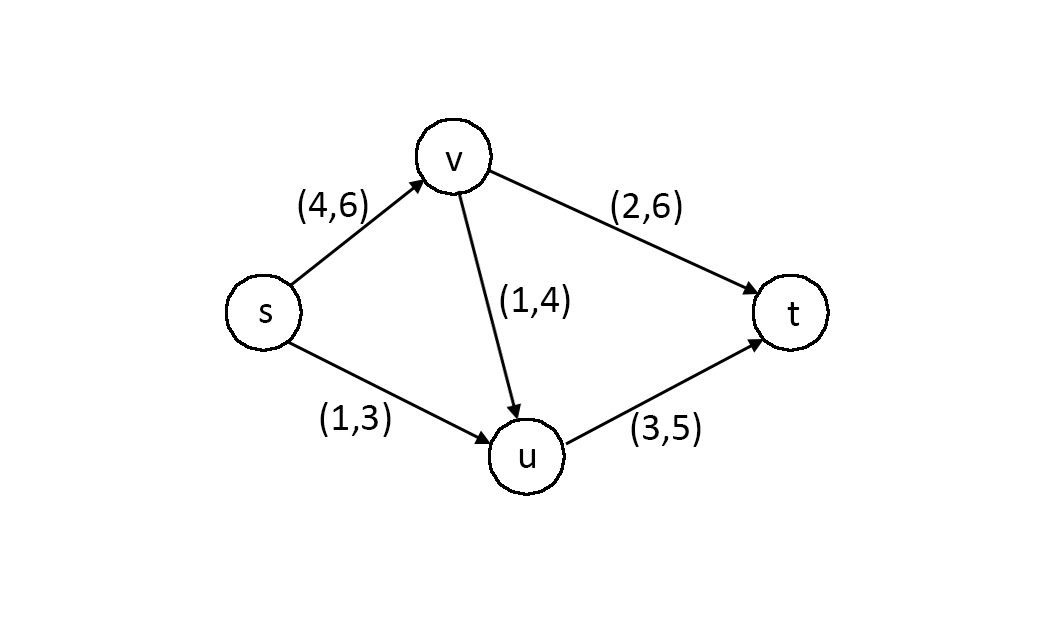
\includegraphics[scale=0.2]{imagenes/min0.jpg}}
	\only<2>{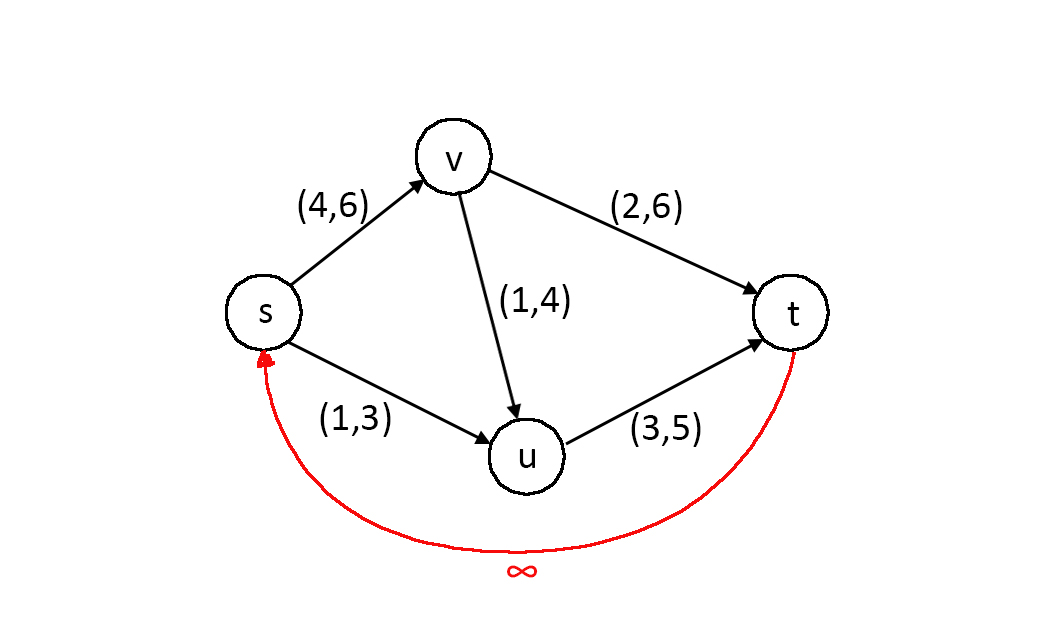
\includegraphics[scale=0.2]{imagenes/min1.jpg}}
	\only<3>{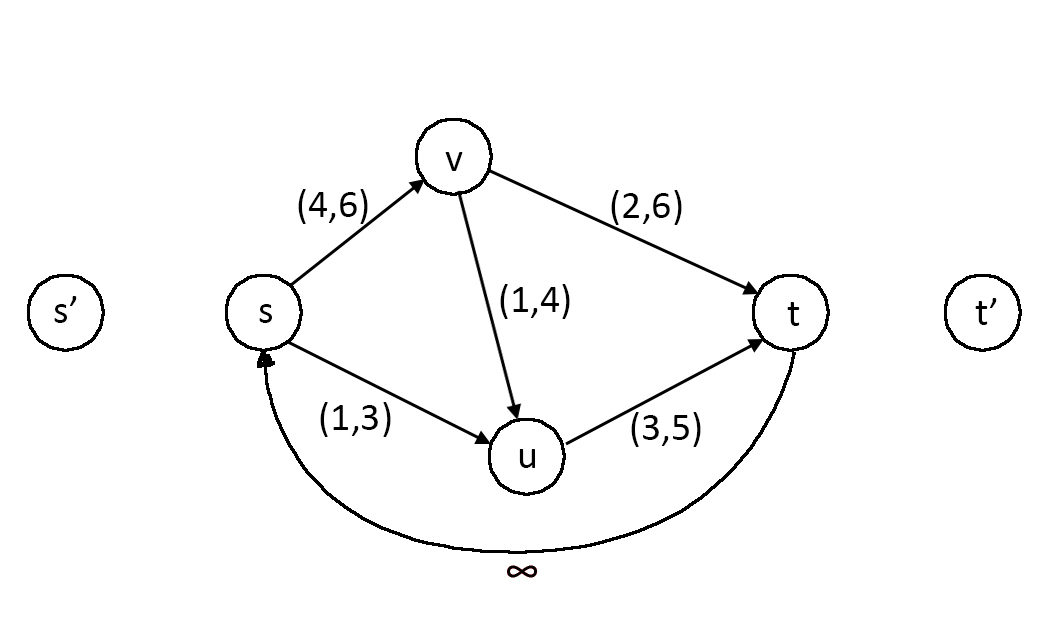
\includegraphics[scale=0.2]{imagenes/min2.jpg}}
	\only<4>{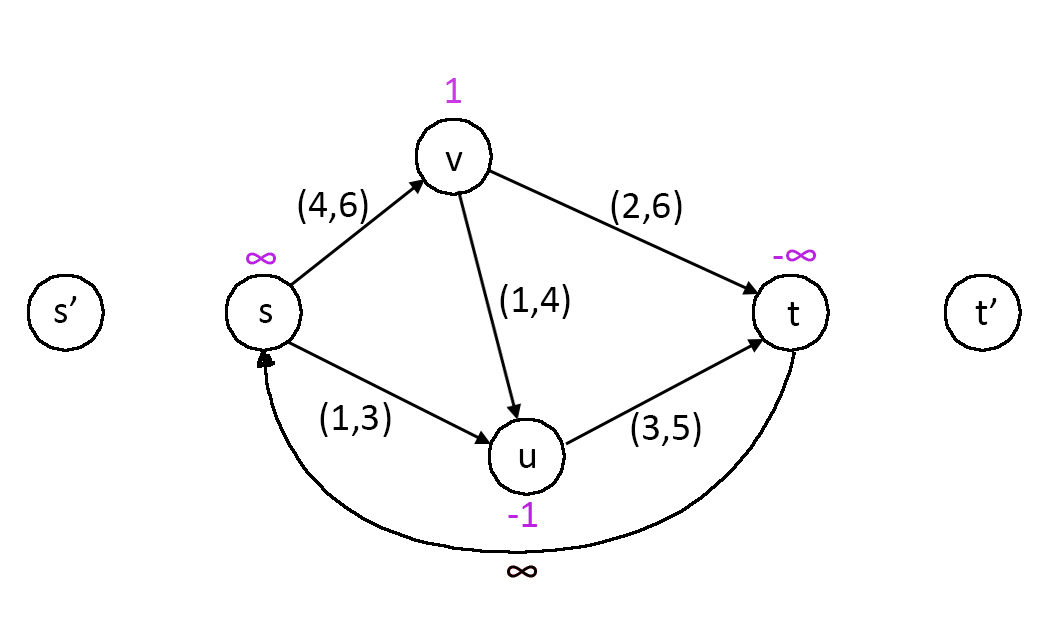
\includegraphics[scale=0.2]{imagenes/min3.jpg}}
	\only<5>{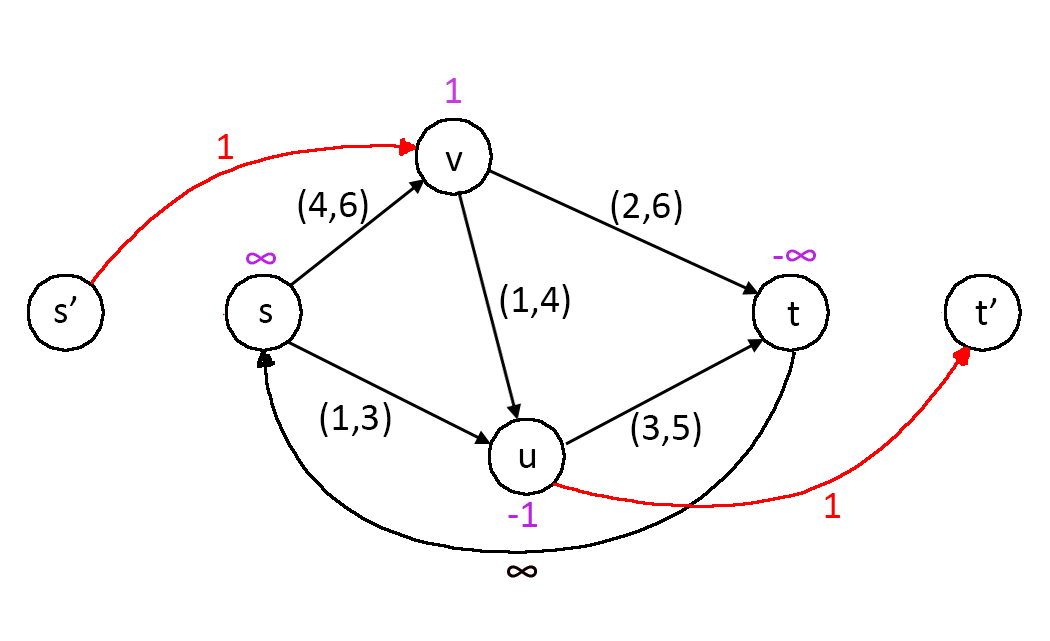
\includegraphics[scale=0.2]{imagenes/min4.png}}
	\only<6>{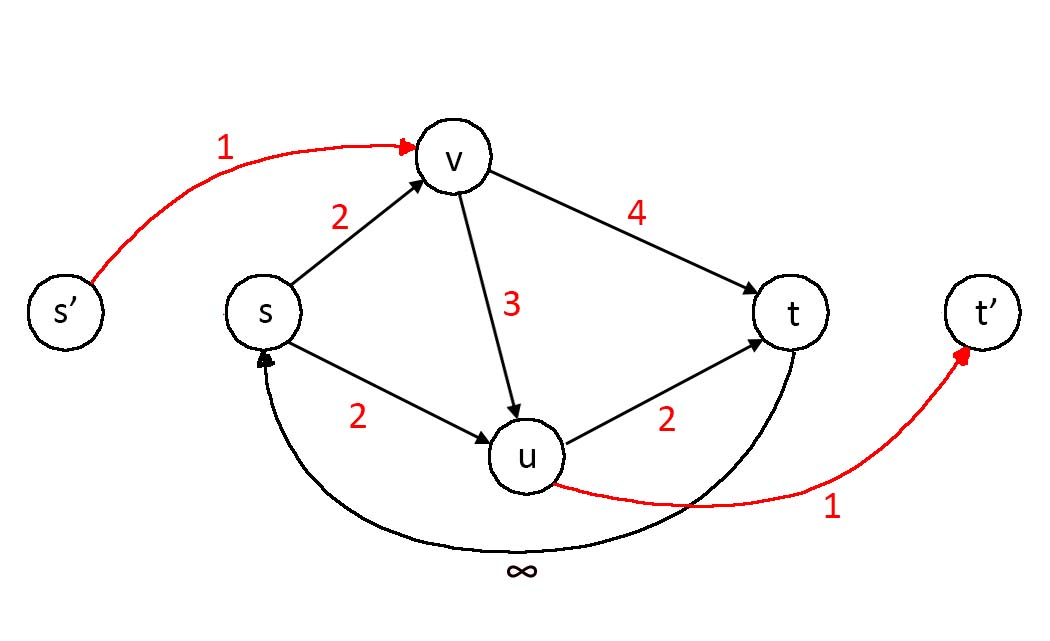
\includegraphics[scale=0.2]{imagenes/min5.jpg}}
	\only<7>{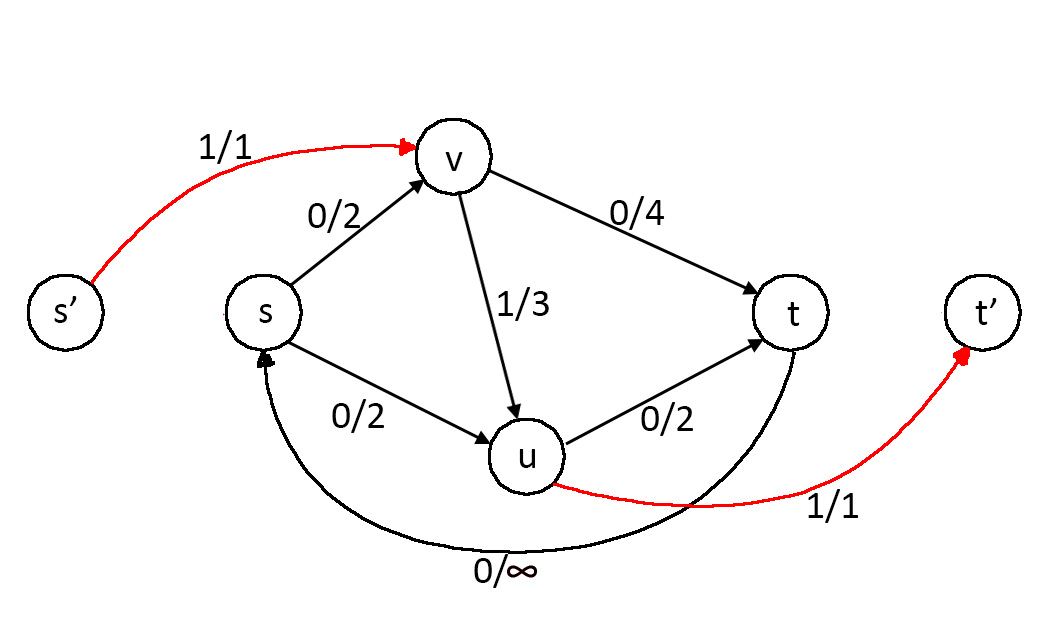
\includegraphics[scale=0.2]{imagenes/min6.jpg}}
	\only<8>{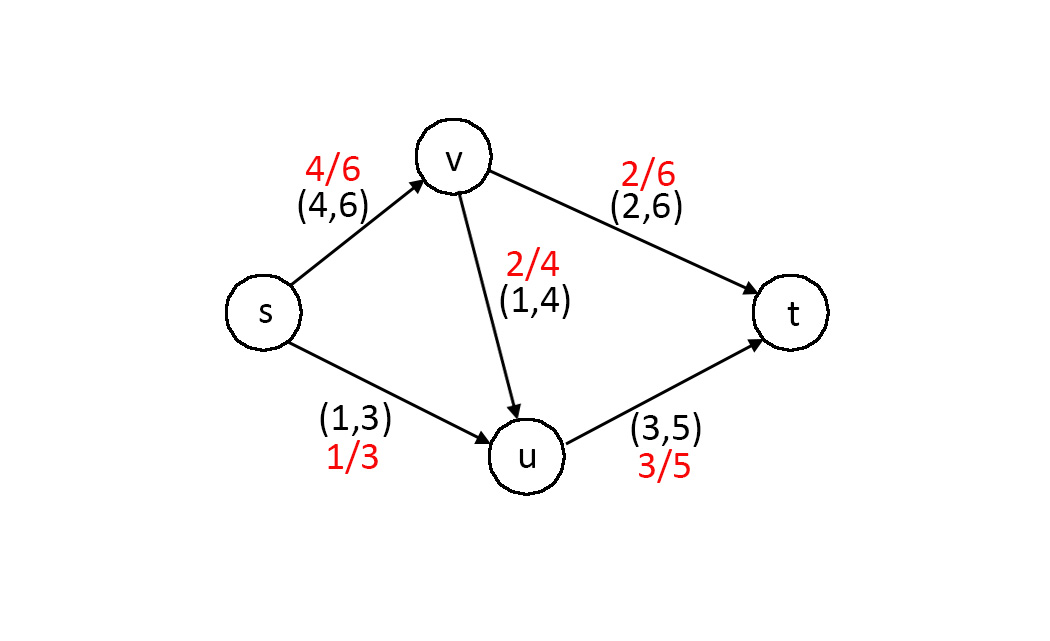
\includegraphics[scale=0.2]{imagenes/min7.jpg}}
	
\end{frame}

\begin{frame}{Ejercicio}
	Se tienen dos conjuntos de enteros, $\mathcal{A}$ y $\mathcal{B}$. Se desea eliminar la menor cantidad de n\'umeros en total de forma que no exista ning\'un n\'umero de $\mathcal{A}$ que divida a alguno de $\mathcal{B}$.
	
	Modelar el problema en t\'erminos de alguna red de flujo adecuada.
	
\end{frame}

% \begin{frame}{Ejercicio 2}
% 	En un juego participan $N$ jugadores, uno de ellos es el hombre lobo. En la primera ronda, cada jugador se\~nala a otros dos jugadores. En la segunda ronda se revela qui\'en es el hombre lobo. 
	
% 	Luego, todos los jugadores restantes deben elegir votar a alguien, pero cada jugador solo puede votar a alguien que haya se\~nalado en la priemra ronda. Despu\'es de esto vota el hombre lobo.
	
% 	Si al finalizar el proceso el hombre lobo es el m\'as votado, entonces todos salvo el hombre lobo ganan. De no ser as\'i, gana el hombre lobo.
	
% 	Sabiendo las elecciones de la primera ronda y qui\'en fue revelado como hombre lobo, modelar el problema de determinar si los jugadores pueden ganarle al hombre lobo en t\'erminos de alguna red de flujo adecuada.   
% \end{frame}

% \begin{frame}{Ejercicio 2}
% 	En el a\~no 2078, Tulio Brondona gobierna el f\'utbol mundial, y decidi\'o que por partido ganado un equipo reciba 2 puntos (el empate y la derrota siguen valiendo 1 y 0 puntos respectivamente).
	
% 	Ya se llevan jugados una serie de partidos. ¿Puede nuestro equipo salir campe\'on?
	
% 	Modelar el problema en t\'erminos de alguna red de flujo adecuada.
% \end{frame}
% \begin{frame}{Contenidos}
%   \setbeamertemplate{section in toc}[sections numbered]
%   \tableofcontents[hideallsubsections]
% \end{frame}





\end{document}

